\documentclass[12pt, a4paper]{amsart}
\usepackage{amsmath}
\usepackage{gensymb}
\usepackage{textcomp}
\usepackage[utf8]{inputenc}
\usepackage[a4paper, margin = 1in]{geometry}
\usepackage{bm}
\usepackage{graphicx}
\usepackage[hyphens]{url}
\usepackage{natbib}

\title[Undergraduate PIV analysis program]{A web-based python PIV analysis program for use in undergraduate laboratory experiments.}
\author[Jacob Sephton]{Jacob Sephton\\ supervised by Prof. Julio Soria}

\begin{document}
\maketitle

\section{Introduction and Aims}
\subsection{Introduction}
Many methods exist for measuring velocity, but many commonly used methods, such as pitot tubes, restriction plates, or turbine meters only measure velocity at a point or as an average across a section, and may affect flow both up and downstream of the measurement device \citep[pp. 109, 469]{munson}. These methods have the advantage of simplicity of measurement, but they cannot be used to determine the behaviour of a broader flow field within a flow: another method is required. 

Particle Image Velocimetry (henceforth: PIV) is one such method. In PIV, marker objects -- usually small spheres -- with neutral buoyancy are introduced to the portion of the flow to be studied \citep{wikipiv}\footnote{While not appropriate for a more in-depth analysis, Wikipedia provides reasonably good high level summaries of most concepts and is cited here for this reason.}. When appropriately sized for a specific flow, these particles will track the bulk motion -- the advection -- of the flow, with a high degree of accuracy. Both the magnitude and direction of the velocity around the particle can then be determined through photography over a known time interval. When many particles are used, the velocity at many points in a flow field can be measured at once, permitting the interpolation of the entire velocity field in a given region of a flow. And, by varying the parameters of the study, like fluid properties, flow rate, particle size, and time interval, flow phenomena at different length and time scales can be modelled. 

In light of these potential benefits, undergraduate laboratory experiments to introduce the method represent an opportunity for students to learn about a powerful analytical technique. Since PIV methods require the processing of large amounts of data, computers are used for analysis, and the software used to do so -- PIV analysis software -- uses a variety of algorithmic and signal processing techniques to do so.

Developing a PIV analysis program for undergraduate use will be the focus of this project. This program will use Dash, a declarative web application framework, and Python code to implement PIV analysis, and make analysing, presenting, and exporting data simple and easy. Dash is a good framework for the development of such an application, as it is open-source and designed to make interface implementation and data display (relatively) painless \citep{aboutdash}. Furthermore, being web-based, Dash provides the capacity for the application to be used remotely on almost any computer. The specific feature requirements and implementation details of the application will be determined as part of the project, and development will be carried out in an iterative fashion to manage complexity. 

PIV software is not new, nor is it inaccessible. OpenPIV, for example, is an open-source PIV analysis package available under the GPL\footnote{Referring to the GNU General Public License, an influential ``copyleft" software license that requires derivative software be made available under it's own terms.} \citep{openpiv}. The difference between this software and that which is currently available will be that this project has an explicit and narrow target application: that of teaching about PIV in an undergraduate lab setting. Such software may be further made relevant by the potential for this undergraduate learning to take place remotely: while the hardware required to capture PIV images may be expensive, the analysis can be performed anywhere.

\subsection{Aims}
This project aims to develop a PIV application with a didactic focus. This will involve:
\begin{itemize}
	\item Determining the specific requirements of the application. Input form, analysis capabilities, and the degree to which the mechanisms of analysis are made visible to the user are all to be determined. This will further involve determining whether physical apparatus needs to be made a part of the development process
	\item Creating a spec and development timeline for the application which prioritises essential features first to ensure that deadlines are met, and identifies worthy extensions to essential features for continued development.
	\item Conducting research to understand the theory behind and parameters of PIV analysis and signal processing to the extent necessary to teach the most important concepts behind them in an engaging way.  This will further involve researching methods for interpreting output of PIV, identifying error sources, limitations, and data transformations that can provide insight into the flow phenomena studied.
	\item Developing tests to evaluate the performance of the application. This may involve comparing application output with other packages using widely used benchmark input, such as the PIV images available on PIV Challenge \citep{pivchallenge}.
	\item Potentially developing a lab script that could be used in conjunction with the application that makes use of the application's features and develops students' understanding of the PIV process. 
\end{itemize}


\section{Methodology}
The methodology for both software development as it pertains to this project and of PIV more generally are discussed in this section.  Software development methodologies are a specific domain of project management practices designed to manage the complexities associated with writing software, and will help ensure that major component of this project succeeds. Meanwhile, it is important to discuss the particulars of PIV from a physical perspective as a basis for developing understanding of the topic and informing design decisions to be made. 

\subsection{Software development}
Since software projects grow in complexity quickly with increasing scope, the field of software engineering has arisen to develop and formalise best practices that make writing functional, easily maintainable, and extensible software something that can be done repeatably and efficiently. Since a major portion of this project concerns the delivery of a software application, the adoption of some of these best practices seems prudent. We will consider development methodology and version control systems as part of this proposal. 

Development methodologies are principle-guided sets of decisions around how software is written that aim to optimise the quality of software along one or more axes. For this project, principal considerations include hard deadlines that must be met, the fact that the conclusion of development must occur well in advance of these deadlines, and the prospect of requirements changing through the course of the project. With these issues in mind, the methodology used for this project will draw from Agile principles. 

Agile software development stresses, among other things, the delivery of working software early and continuously \citep{agile}. To do this, software is reduced to its minimal feature set to begin with, then built upon iteratively. The facts that working software is produced as early as possible, and feature addition decisions do not need to be made until work on that feature actually commences makes this an appropriate school of development to draw from for this project, helping to meet deadlines and deal with requirement flux.

Informing this is the development of a functional specification (spec) early in the process. Per \citep{joelspecswhy}, advantages of doing this include the fact that design decisions that have to be made anyway can be made before code is written, avoiding wasted effort, and that a detailed spec allows development work to be scheduled, helping to deliver the best possible application by the deadline. A spec will be developed for this project similar to one described by \citep{joelspecshow} detailing how the software will work from the user's perspective. This will inform the technical decisions made further along. 

Software will be used to assist the development process. Firstly, Git, a version control system, will be used to back-up and track changes to the codebase over time. It permits branched feature development while always having access to the last functional version of the software, and these features can be merged back into the existing main version of the software, even if changes have been made to the main version since the branch occurred \citep{bilschakvcs}. Secondly, task tracking software Jira \citep{jira}, which is designed to facilitate an Agile development methodology, will be used for organisation. 



\subsection{PIV methodologies}
PIV typically involves the study of flow in a single plane of a broader system. To accomplish this, a planar strobe lighting setup is common, with a strobe or laser firing through a cylindrical lens, which spreads the beam out along one axis, and then through a spherical lens which focusses the light to a thin sheet at the area of study. Arising from this is the possibility of parallax error in measurement, from lit particles that are closer or further away from the lens than the centre of the light plane. Another error source arising from the planar nature of most PIV analyses is motion perpendicular to the imaging plane, which can lead to incorrect conclusions being drawn if not accounted for. This does mean that PIV is best applied when the imaging plane can be made to closely match the predominant flow directions in the area of study. For more complicated flows, stereo imaging can be used to carry out PIV in three dimensions, albeit with added complexity and cost. 

One potential error source in PIV is tracking error between particles and the flow field. This makes particle and flow medium selection an important part of carrying out PIV analysis. In Stokes flow, with particle Reynolds numbers, Re$_p$ (\ref{repart}), less than 1, the Stokes number, Stk, can be given by (\ref{stk}). The Stokes number describes the relationship between the characteristic time of the flow and the response time of a particle in that flow, and thus is highly relevant when considering PIV particle parameters. Higher Stk implies either a high particle response time, or a proportionately high velocity-to-feature size ratio and thus suggests that the motion of the particle will not capture the full velocity profile of the flow \citep{wikistokes}.


\begin{equation}\label{repart} \textnormal{Re}_p = \frac{\rho_f u d_p}{\mu} \end{equation} 

	\begin{equation}\label{stk} \textnormal{Stk} = \frac{t_0 u}{l_0} | t_0 = \frac{\rho_p d_p^2}{18\mu}\end{equation}

In these equations, $\rho$ is density of the fluid or the particle, $u$ is fluid velocity, $d_p$ is particle diameter, $\mu$ is fluid viscosity, $t_0$ is particle response time, and $l_0$ is the characteristic length of the flow being studied. Compromise must be made between minimising $t_0$ through small particle $d$ and difficulty in imaging small particles. Much more goes into the consideration of particle and fluid parameters than can be contained within the scope of this proposal, but this provides an example.  

One last point of note are signal processing techniques used in PIV. All PIV analysis requires the interpretation of images to generate velocity fields, and automated methods of doing so vary depending on the images captured. Some PIV, especially using older cameras, relies on two strobes within a single exposure. Here, autocorrelation is used to determine velocity from particle displacement within one image. Newer PIV often uses multiple exposures, with the benefit of being able to identify flow direction: PIV of this sort uses cross-correlation between images. Cutting-edge techniques are investigating the use of machine learning to correlate images with velocity fields, with the benefit of improved velocity field resolution \citep{wikipiv}.


\section{Project plan}

The project is broken into stages for planning purposes. Appendix \ref{timeline} shows the proposed timeline for the project, detailing when each stage should be started and finished, contextualised within the rest of the project. An elaboration on each stage described therein follows.

\subsection{Project proposal}
You're reading it! This stage involves not just the creation of the report, but also initial broad research undertaken to gain an understanding of the project and its future direction. Deliverables include this report, a risk assessment for project work, and an understanding of the project's future direction.

\subsection{Learning Python and Dash}
This stage involves completing the Dash tutorial \citep{dashtut} and familiarising myself with the Python programming language. Subtasks involve setting up a source control repository for project work and a development environment on my computer. This task is mostly complete, and I'll finish the tutorial over the mid-semester break. 

\subsection{Requirements determination}
In this stage the specific requirements of the app will be defined and clarified. What features must the app have? What non-essential features should be prioritised. How should it work, and how will the design decisions made serve the aim of introducing PIV to undergraduate students. This stage will also involve research into specific algorithms that can be used in PIV, and reading to understand both PIV and the signal processing theory that makes it possible. This stage strongly informs the spec that will be developed in the next stage.

\subsection{Application specification}
Here, a specification document will be produced for the application. It will define the proposed architecture, and all of the features the app needs to have to be considered complete. It will also define future feature development, prioritising non-essential features that will have the biggest impact on the usefulness of the application. Tests will be developed to measure application performance. This document will inform the implementation of the software through the middle of the project. A lab script may be treated as a feature of the application for project management purposes. 

\subsection{Progress report}
A report detailing findings in the project to this point will be produced. It will contain the findings of research to this point, decisions made around design and features, and the specification document, likely abridged in some fashion. The progress report will also include some information on how implementation is proceeding, and perhaps some demonstration of any software features implemented, if possible. 

\subsection{Implementing the specification, followed by iterative development}
The actual programming will be done in this stage. See methodology section for more detail.

\subsection{Final report and research paper}
The final report and research paper will be started early, in the mid-year break. The final report will detail all outcomes of the project: the findings of research carried out, how software was implemented, how the finished software performs, and will evaluate the work carried out in terms of the aims of the project. The research paper will investigate an area related to the project, likely informed by research carried out in earlier stages. The aim will be to build both of these documents over the course of semester two, with the first draft of each due at a self-set deadline at the end of week 8 and week 9 respectively. Having these done early will avoid an end-of-semester crunch. 

\subsection{Shooting and editing project video}
The project video will be started as the development phase winds down, and should present the main findings of the final report in an engaging short presentation. A demonstration of the application will feature, and I will talk about the process of research and development that went into it. The self-set deadline at the end of the mid-semester break is the last deadline in the project prior to official deadlines, leaving room for the polishing stage,

\subsection{Polishing}
At this point, all project deliverables should be complete, at least to the first draft. This stage is where edits, final corrections, and any necessary supplementary information are added to the reports and videos. Two weeks of polishing time is allocated for the video, and three for the two reports. This stage should allow all deliverables to be ready well in advance of their deadline. 





\bibliographystyle{apa-good}
\footnotesize{
\bibliography{refs}
}

\pagebreak
\appendix

\section{Proposed project timeline}\label{timeline}
\begin{figure}[h]
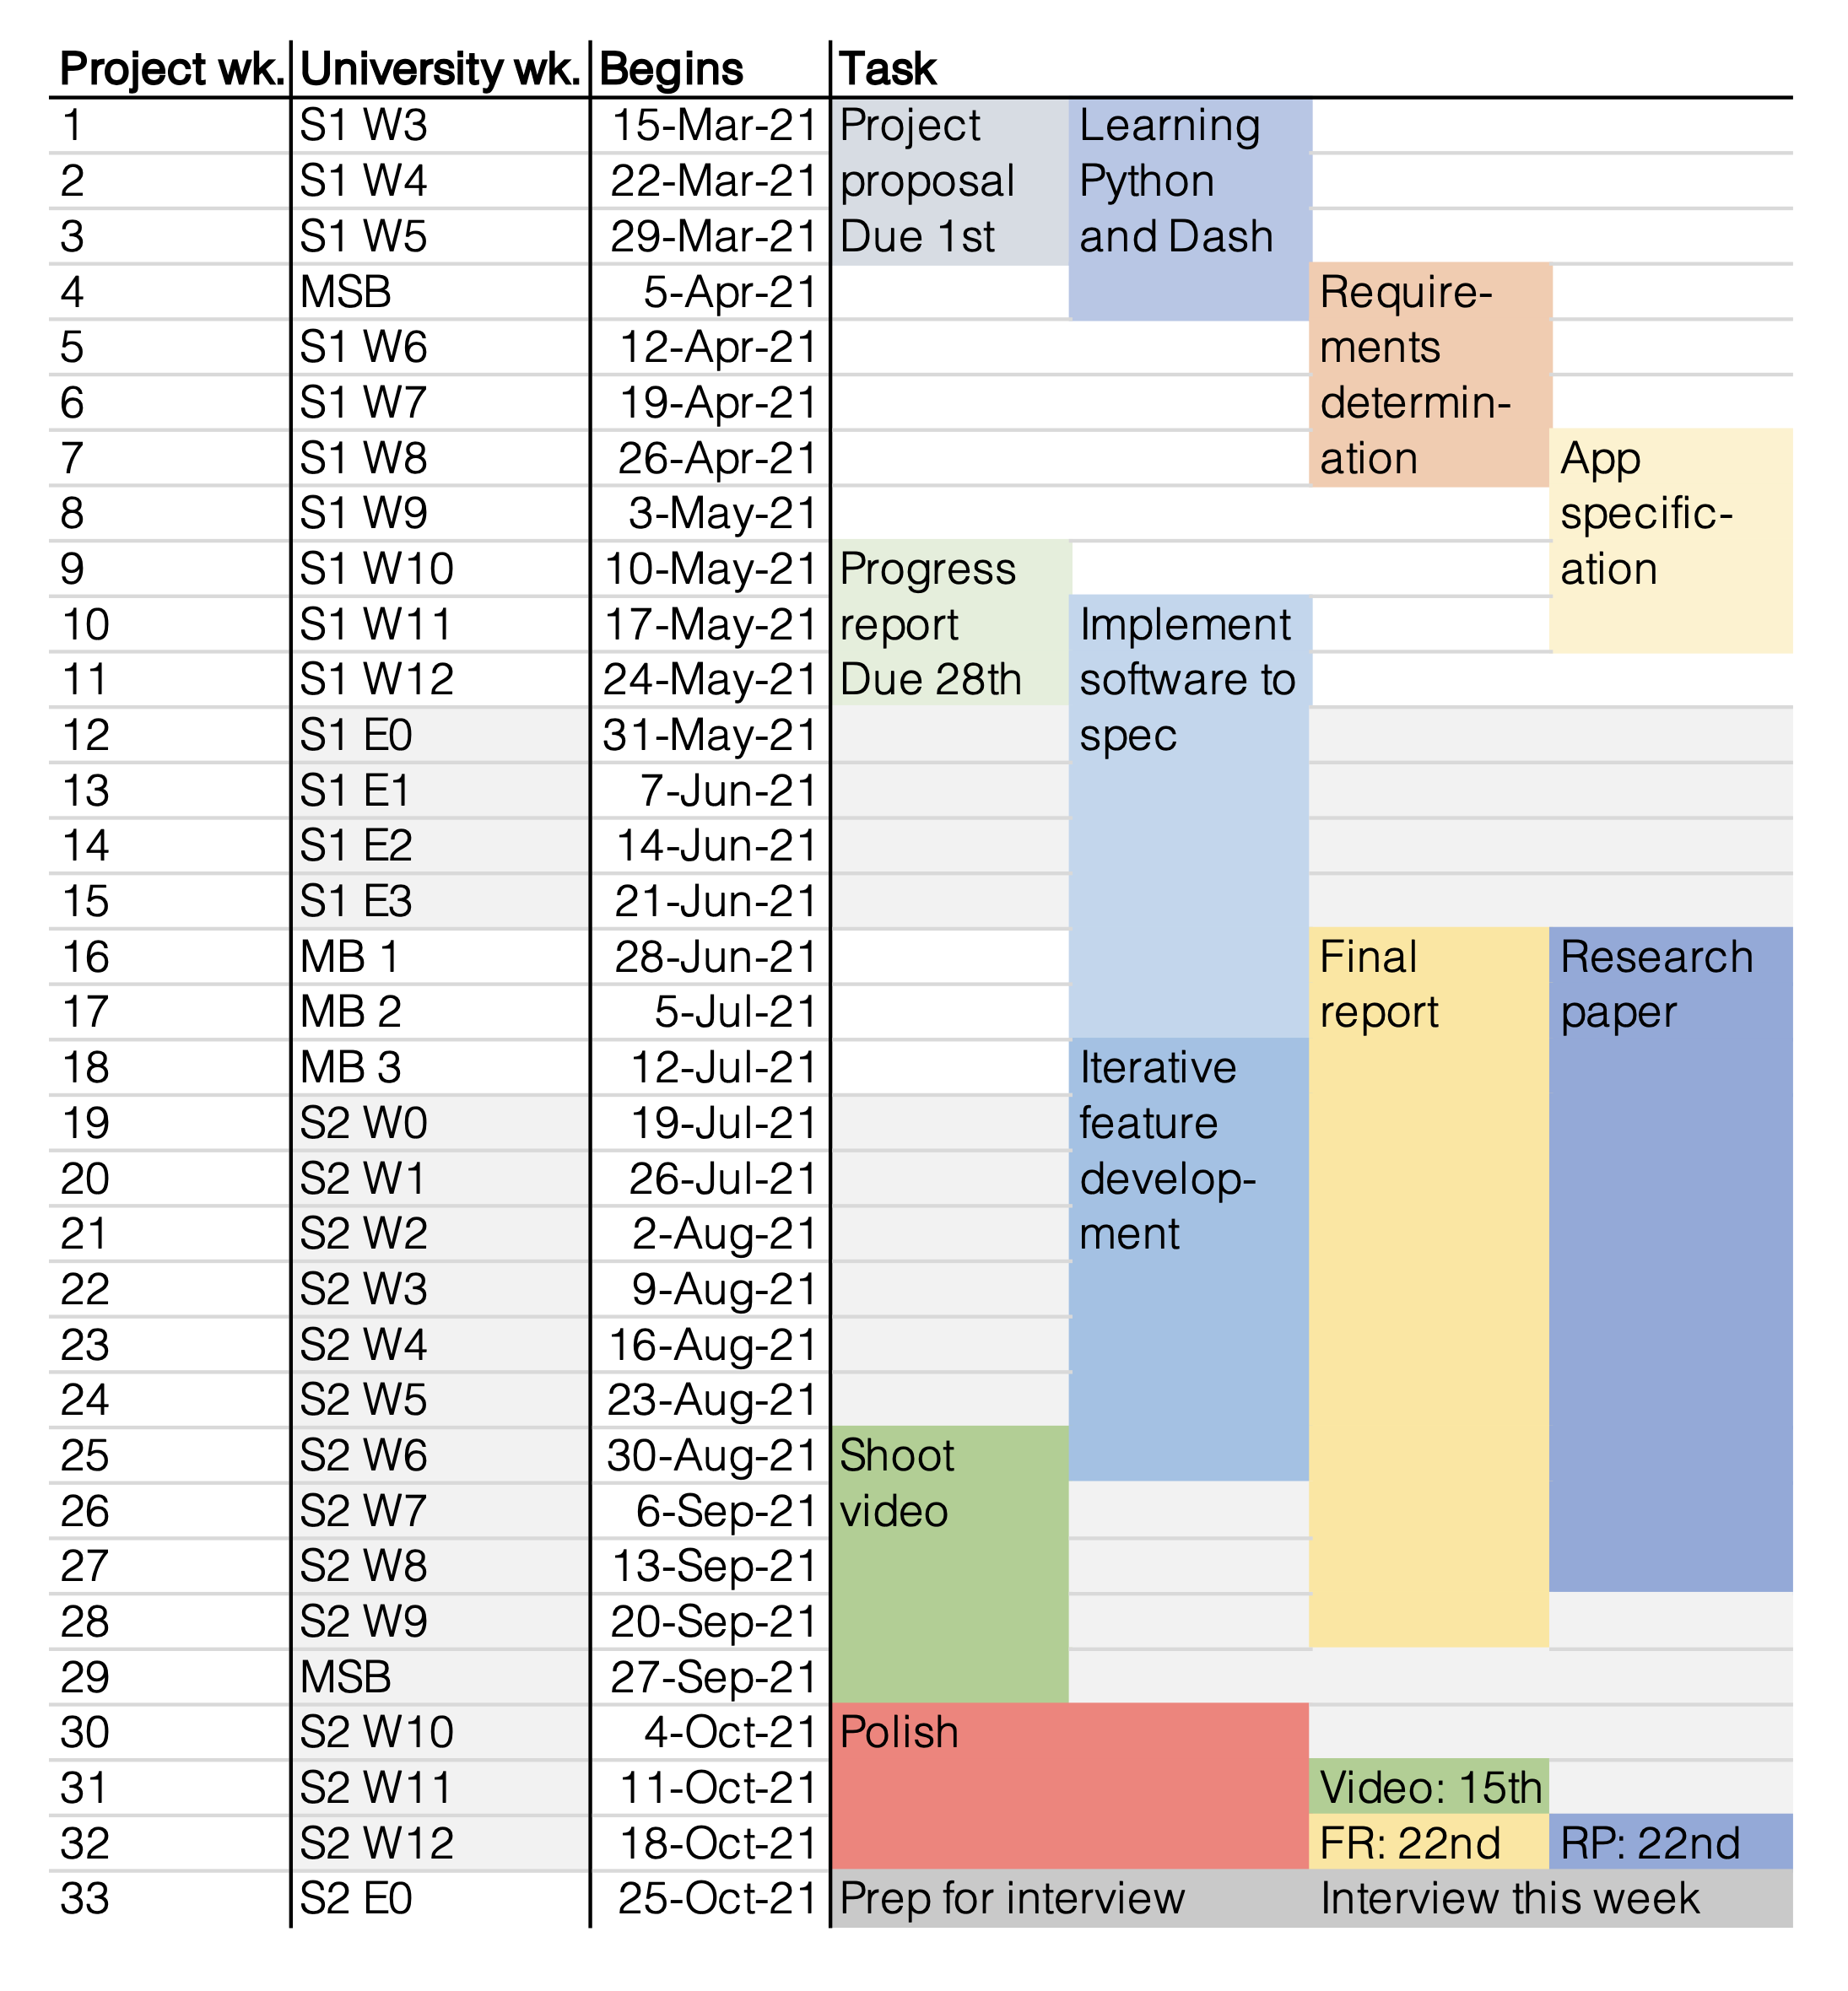
\includegraphics[width = 16cm]{timeline.png}
\end{figure}

\section{Risk assessment}
See following pages.


\end{document}